%!TEX root = Bericht.tex
\graphicspath{{graphics/HMI/}{graphics/control_modes/}}
\chapter{The different Control Modes}
\label{cha:DifferentControlModes}

\textbf{\textit{About the need of different modes, the requirements of image capturing and overview of the realized modes}} \\

As mentioned in section \ref{sec:system overview}, one of \textsc{Skye}'s unique properties are the decoupled 6DOF of space. This means, the system has the possibility to turn around an arbitrary axis while moving to any direction. This ability has to be used to fulfill the operation tasks in an optimal way. An intuitive handling for the pilot has to be granted in any way. \\ 
The first approach is to provide a manual control mode that allows to pilot the 6DOF directly by the operator. A detailed description will be given in section \ref{sec:manualControlModes}. \\ 
In contrast to the unrestricted control possibilities for manual control, a more autonomous control would allow the pilot to focus on a specific motion, e.g. the orientation of the camera. Therefore, a part of the 6DOF motion of \textit{Skye} will be automated\footnote{The prototype designed for this project does not include any environment detections. Therefore, autonomous control with obstacle detection will not be possible yet.}. In section \ref{sec:automaticControlModes} this is described in more detail. Furthermore, a basic \textit{test phase} control mode lets the operator directly access the 8 actuations individually. Table \ref{tab:control_modes} gives an overview of the control modes. Those actual realization is presented in chapter \ref{cha:findHardSoftSolution}.

\begin{table}[h]		% [H] indicates that the table should be right here.
	\begin{tabular}{c c c c c} %{p{0.16\textwidth}p{0.16\textwidth}p{0.16\textwidth}p{0.16\textwidth}p{0.16\textwidth}}	% add p{size_of_column} for every new column you'd like to have. If you put a | between the p then there is a vertical line between the columns. 
	Test Phase 		& Direct Control 	& Assisted Control 	& Half Automatic	& Full Automatic  \\
	\toprule[1.25pt]				%define the line thickness of the top rule
	Thrust 1		& Thrust $x$	& Velocity $x$	& Velocity	& Velocity	\\
	Thrust 2		& Thrust $y$	& \textit{Velocity $y$}	& Rotation $x$	& Rotation $x$\\
	Thrust 3		& Thrust $z$	& \textit{Velocity $z$}	& Rotation $y$	& Waypoints	\\
	Thrust 4		& Moment $x$	& Rotation $x$	& Rotation $z$	&	Camera target\\
	Direction 1		& Moment $y$	& Rotation $y$	& Waypoints	&	\\
	Direction 2		& Moment $z$	& Rotation $z$	&		&	\\
	Direction 3		& 		& 		&		&	\\
	Direction 4		& 		& 		&		&	\\

	\bottomrule[1.25pt]
	\end{tabular} 
	\caption[The different control modes]{With the control modes, different inputs are given to the controller. The inputs in \textit{italic} are not available for \textit{Assisted RC  Control}.}
	\label{tab:control_modes}
\end{table}

\section{Manual Control Modes}
\label{sec:manualControlModes}
\textit{Direct Control and Assisted Control}
\subsubsection{Test Phase} 
As \textsc{Skye} was built as an prototype in parallel to this thesis, the overall functionality of the system had to be checked piecewise. The \textit{test phase} control mode was therefore designed to test the propulsions behaviour. The number of revolutions as well as the reference orientation of each of the four actuation units can be set individually\footnote{In \cite{schaffnervu} referred to as input for the \textit{Thrust Section} and \textit{Positioning Section} respectively.}.

\begin{figure}[H] % [H] steht dafür, dass das Bild genau hier im Text sein soll.
	\begin{center}
		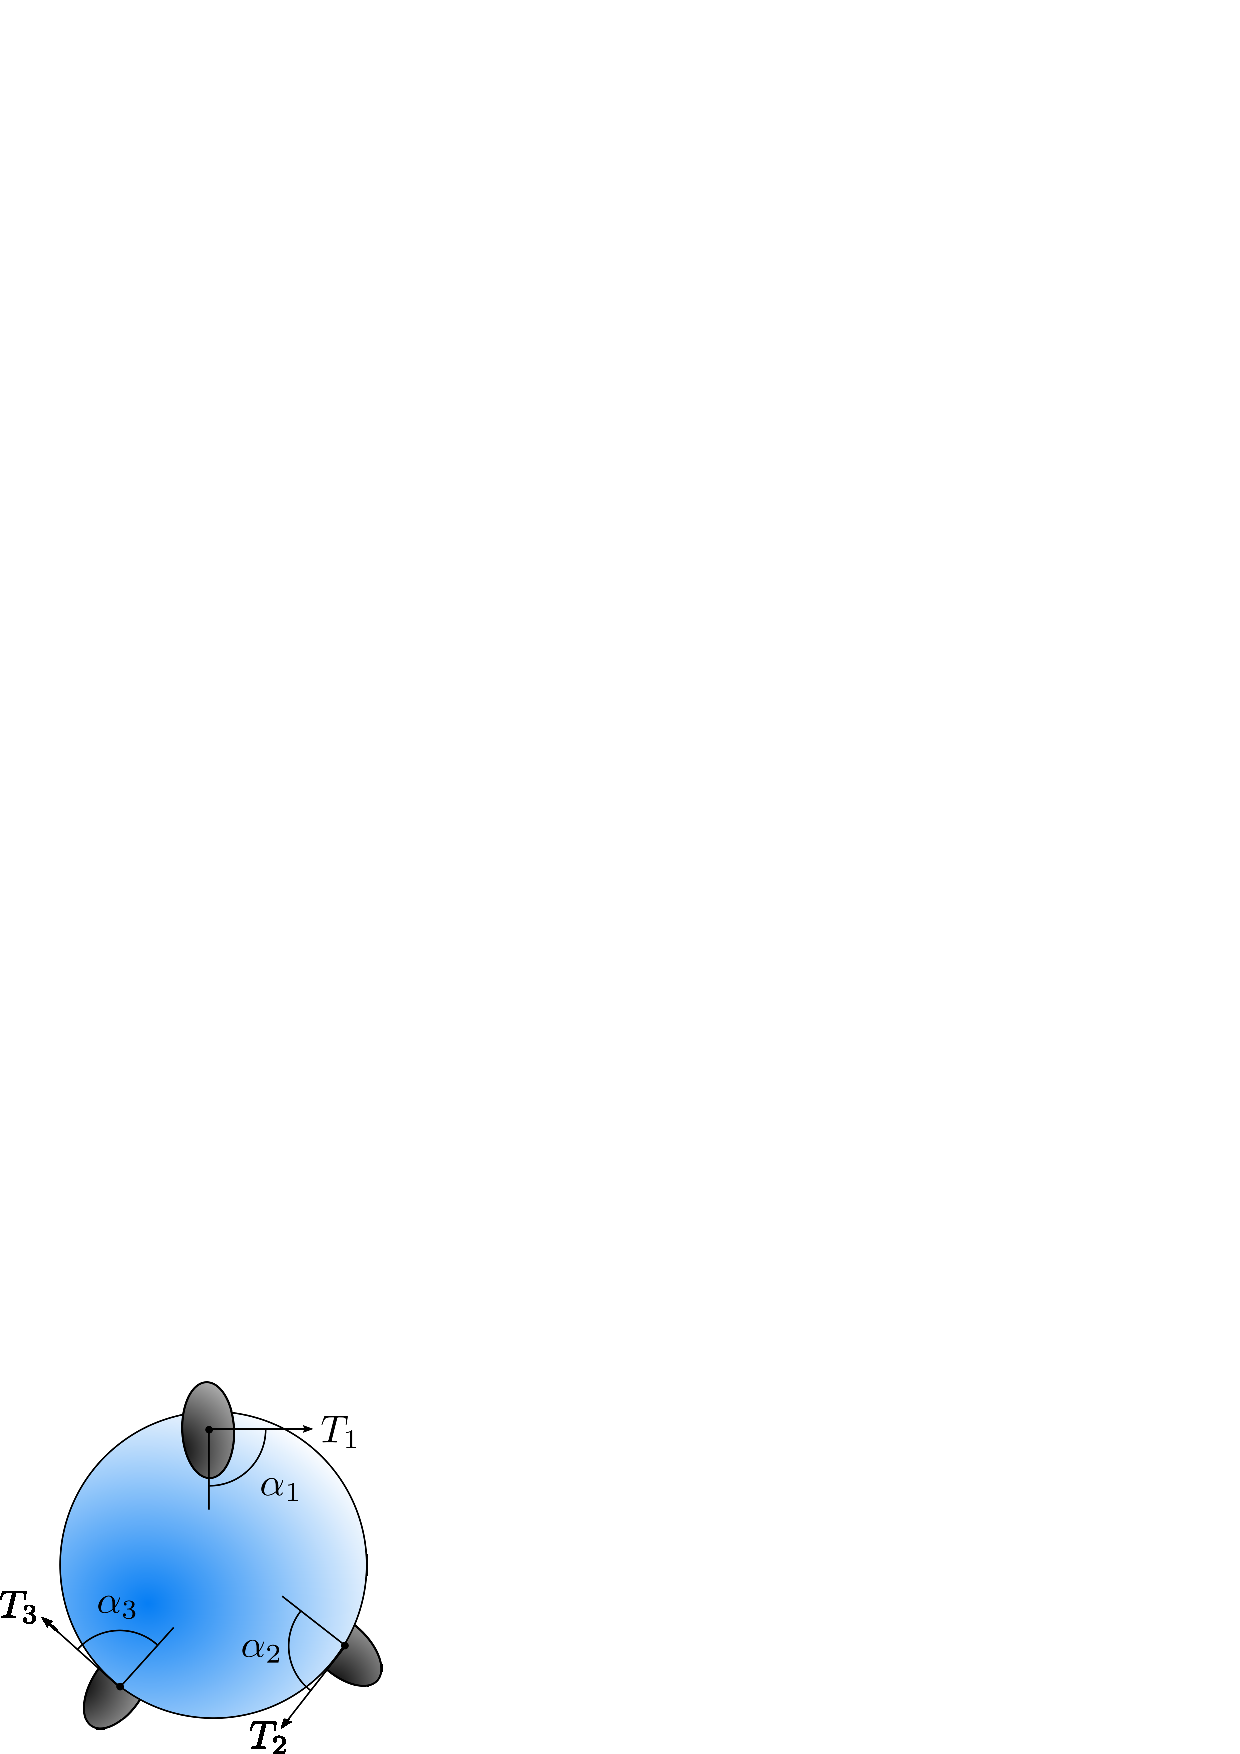
\includegraphics[width=0.3\textwidth]{TPC.pdf}
		\caption[Test Phase]{Test Phase}  
		\label{fig:test_phase}		
	\end{center}
\end{figure}


\subsubsection{Direct Control} 
A second control mode that mainly intends to verify the system's properties is the \textit{direct control} mode where the operator sets the desired force and moment vectors. This 6DOF control therefore needs the transformation of the forces and moments to the 8 actuations\footnote{See \cite{schaffnervu} for details about the optimization criteria for the motor allocation.} only. No information about the system's properties and states are needed. The pilot's input is interpreted as the force and moment components in body fixed coordinates. As the camera system (the eye of \textsc{Skye}) represents the most recognisable orientation, the coordinate frame was aligned to the camera's orientation. This is illustrated in figure \ref{fig:direct_control}, where ${e_x^c, e_y^c, e_z^c}$ represents the camera orientated frame ($e_x^c$ collinear with the camera axis, $e_y^c$ heading left, $e_z^c$ bottom).

%\begin{figure}[H] % [H] steht dafür, dass das Bild genau hier im Text sein soll.
%	\begin{center}
%		\includegraphics[width=0.37\textwidth]{DC.pdf}
%		\caption[Direct control]{Direct Control}  
%		\label{fig:direct_control}
%	\end{center}
%\end{figure}

\begin{figure}[H]		
	\small{
		\begin{center}
			\parbox{0.36\textwidth}{\centering 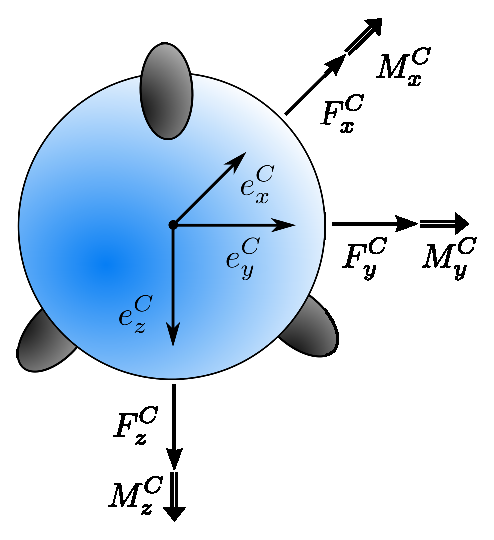
\includegraphics[width=0.36\textwidth]{DC}
			 Direct Control}
			\hspace{0.1\textwidth}			
			\parbox{0.36\textwidth}{\centering 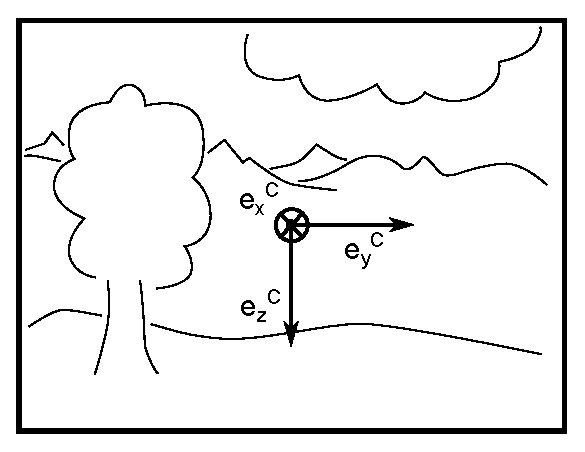
\includegraphics[width=0.36\textwidth]{CameraFrame}
			Camera Frame}
	\caption[Assisted Control]{Direct Control (left) and the orientation of the camera frame in relation to the camera's field of view (right).}
		\label{fig:direct_control}
		\end{center}
	}			
	\vspace{4.5mm}
\end{figure}


\subsubsection{Assisted Control} 
The \textit{direct control} mode demands well trained skills to properly navigate \textit{Skye}. This is especially due to the low damped rotation \cite{weichart} and the symmetrical appearance of the system. To eliminate the first reason, a stabilizing attitude controller is needed. To remedy the second issue, the translational inputs can be interpreted in a earth fixed coordinate frame. By using a proper state estimation, the pilot's commands can directly be interpreted as velocities and angular velocities respectively\footnote{See \cite{meiermueri} for the state estimation and controller design.}.

\begin{figure}[H]		
	\small{
		\begin{center}
			\parbox{0.36\textwidth}{\centering 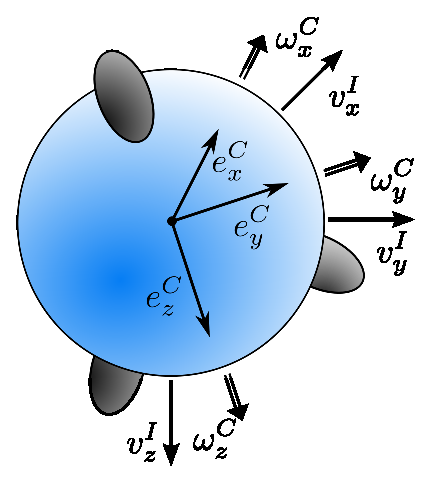
\includegraphics[width=0.36\textwidth]{AC}
			 Assisted Control}
			\hspace{0.1\textwidth}			
			\parbox{0.36\textwidth}{\centering 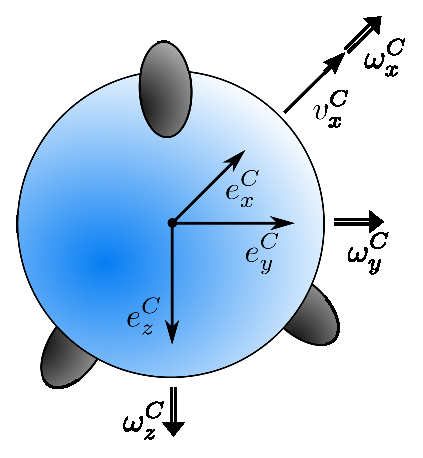
\includegraphics[width=0.36\textwidth]{RC}
			Assisted RC Control}
	\caption[Assisted Control]{Assisted Control with controlling six (left) and four (right) stabilized degrees of freedom.}
		\label{fig:assisted_control}
		\end{center}
	}			
	\vspace{4.5mm}
\end{figure}

\section{Automatic Control Modes}
\label{sec:automaticControlModes}
\textit{Half Automatic Control and Full Automatic Control}

\subsubsection{Half Automatic Control}


\begin{figure}[H] % [H] steht dafür, dass das Bild genau hier im Text sein soll.
	\begin{center}
		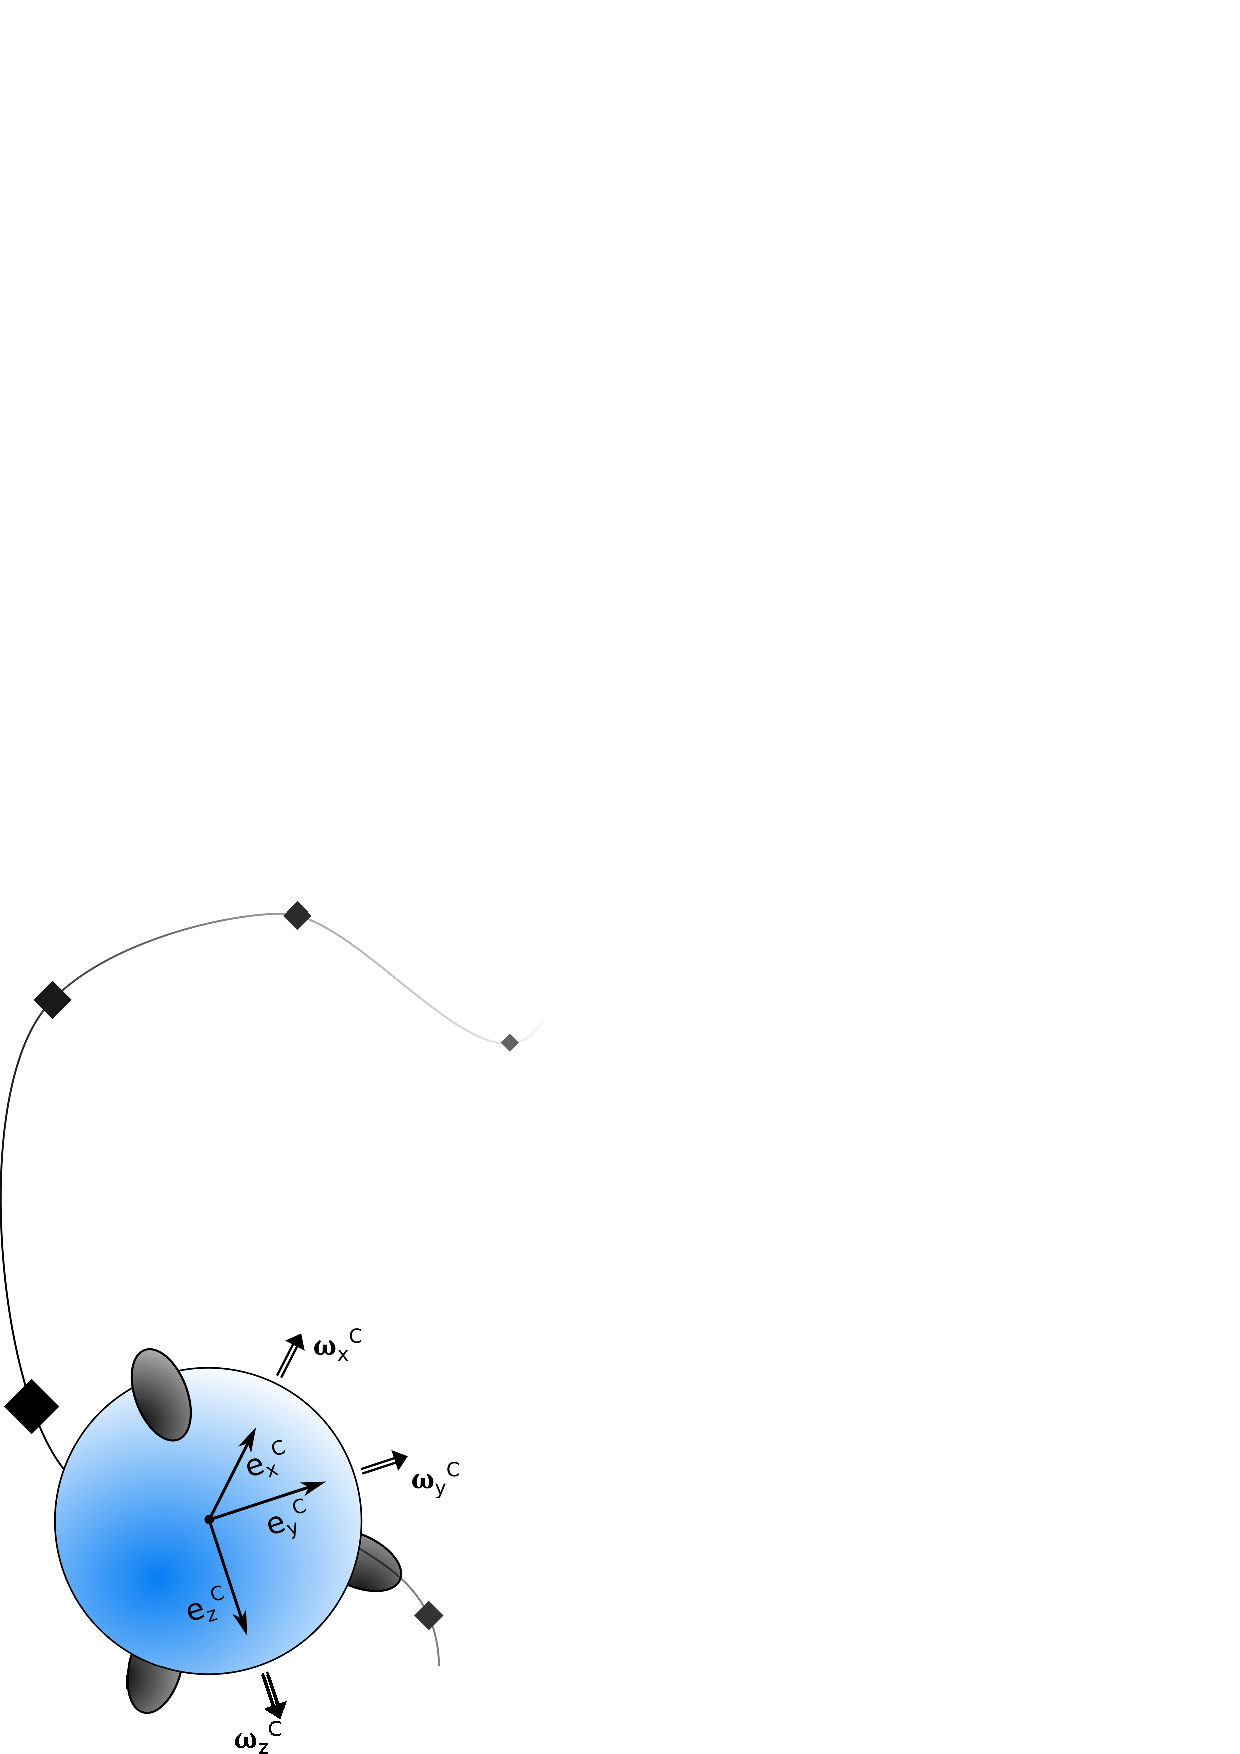
\includegraphics[width=0.4\textwidth]{HAC.pdf}
		\caption[Half automatic control]{Half Automatic Control}  
		\label{fig:half_automatic_control}		
	\end{center}
\end{figure}

\subsubsection{Full Automatic Control}
\begin{figure}[H] % [H] steht dafür, dass das Bild genau hier im Text sein soll.
	\begin{center}
		\includegraphics[width=0.4\textwidth]{FAComega.pdf}
		\caption[Full automatic control]{Full Automatic Control.}  
		\label{fig:full_automatic_control}		
	\end{center}
\end{figure}